
\lecture{10}{Entropy and Heat}{Qiang Zhu}{scribe-name1,2,3}


\section{Mechanical Equilibrium and Pressure}
In the last lecture, we just learned the relation between $S$ and $T$, is there any analogy between $S$ and $P$.

\begin{figure}[h]
\centering
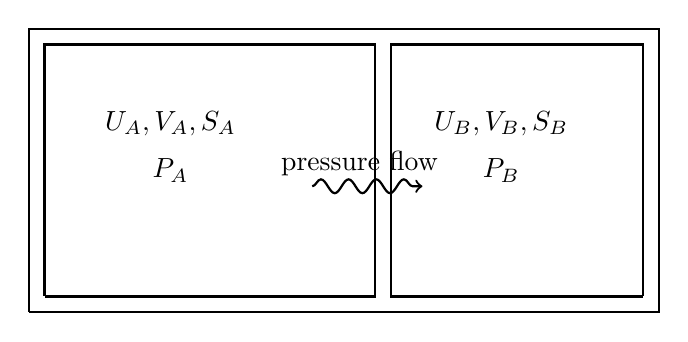
\begin{tikzpicture}[thick]
\draw (0,0.4) -- (8,0.4) -- (8,4) -- (0,4) -- (0,0.4);
\draw (0.2,0.6) -- (4.4,0.6) -- (4.4,3.8) -- (0.2,3.8) -- (0.2,0.6);
\node at (1.8,2.8) {$U_A, V_A, S_A$};
\node at (1.8,2.2) {$P_A$};
\draw (7.8,0.6) -- (4.6,0.6) -- (4.6,3.8) -- (7.8,3.8) -- (7.8,0.6);
\node at (6.0,2.8) {$U_B, V_B, S_B$};
\node at (6.0,2.2) {$P_B$};
\draw [->,decorate,decoration=snake] (3.6,2) -- (5.0,2) node [above, xshift=-0.8cm]{pressure flow};
\end{tikzpicture}
\caption{A schematic pressure flow between two gases.}
\end{figure}

Again, we start from the condition when the system reaches its equilibrium,
\begin{equation} \label{entropy} 
\frac {\partial{S_\text{total}}} {\partial{U_A}}=0     ~~~~~~~~ \rightarrow~~~~~~~~  \frac {\partial{S_\text{total}}} {\partial{V_A}}=0
\end{equation}
as, $S$ is the function of $U$ and $V$.

We already applied the 1st condition in the previous lecture. How about the 2nd condition? 
\begin{equation} \label{entropy} 
\frac {\partial{S_A}} {\partial{V_A}} +  \frac {\partial{V_B}} {\partial{V_A}} =0     ~~~~~~~~ \rightarrow~~~~~~~~  
\frac {\partial{S_A}} {\partial{V_A}} =  \frac {\partial{V_B}} {\partial{V_B}} 
\end{equation}

What's the physical meaning of $\partial{S_A}/\partial{V_A}$? \\
If we dig a bit on the units, we will find $\partial{S_A}/\partial{V_A}$ has a unit of N$\cdot$m/K, about $P/T$ hence we guess
\begin{equation} \label{entropy} 
\frac {P}{T} =  (\frac {\partial{S}} {\partial{V}})_{U,N}     ~~~~~~~~ \rightarrow~~~~~~~~  
P = T (\frac {\partial{S}} {\partial{V}})_{U,N}
\end{equation}

Recall that we know how to calculate $S$,
\begin{equation} S = Nk\text{ln}V + 3/2Nk\text{ln}U - Nk\text{ln}(f(N)) \end{equation}
\begin{equation} P = T(\frac {\partial{S}} {\partial{V}})  = \frac{NKT}{V}\end{equation}
\begin{equation} PV = NkT \end{equation}
Again, we proved the ideal gas law.

\section{Thermodynamic Identity}
From the above sections, it seems that $\Delta{S}$ can be divided into two parts, 
\begin{enumerate}
\item $\Delta{U}$, to account for the heat flow
\item $\Delta{V}$, to account for the pressure flow
\end{enumerate}

Let's say,
\begin{equation} \Delta{S} = (\frac {\Delta{S}}{\Delta{U}})\Delta{U} + (\frac {\Delta{S}}{\Delta{V}})\Delta{V}  \end{equation}
Suppose each step is very small, we use 
\begin{equation} dS = (\frac{\partial S}{\partial U})dU + (\frac{\partial S}{\partial V})dV  \end{equation}
\begin{equation} dS = \frac{dU}{T} + \frac{PdV}{T}  \end{equation}
\begin{equation} TdS = dU + PdV  \end{equation}
\begin{equation} dU = TdS - PdV  \end{equation}
This is {\bf Thermodynamic Identity}
If you compare it with the 1st law, it just substitute $TdS$ as $Q$, which is actually the old definition of entropy.
\begin{enumerate}
\item $\Delta{U}=0$, $dU=TdS$
\item $\Delta{V}=0$, $TdS=PdV$
\end{enumerate}

{\bf Exercise}
Under constant entropy
\begin{equation} (\frac{\partial S}{\partial U})dU + (\frac{\partial S}{\partial V})dV = 0 \end{equation}
\begin{equation} dU = -PdV \end{equation}
isentropic = quasistatic + adiabatic \\
\begin{equation} \Delta{S} = S_f-S_i = \int^{T_f}_{T_i} \frac{C_P}{T} dT \end{equation}
$S(300K)$ = $S(0K) + C_P \int^{300}_{0} \frac{1}{T} dT$ = 5.8 + 3.5*8.31*ln(300) = 173.89 J/K.\\
This value looks much smaller than the reference value in the appendix (197.67 J/K), because of constant volume assumption is not realistic.
A more realistic solution is
\begin{equation} \Delta{S} = C_V\text{ln}\frac{P_B}{P_A} + C_P\text{ln}\frac{V_B}{V_A}\end{equation}
when you consider $Q = U-W$.

\begin{equation} \Delta{S} = \frac{Q}{T} ~~~~~~~~\text{quasistatic}\end{equation}
\begin{equation} \Delta{S} > \frac{Q}{T} ~~~~~~~~\text{in practice}\end{equation}

\begin{enumerate}
\item Very faster compression
\item free expansion
\end{enumerate}



\section{Homework}
Problem  3.5, 3.8, 3.11, 3.14, 3.16, 3.27, 3.30, 3.31, 3.32, 3.33


